\subsubsection{Dashboard}

Dashboard được thiết kế trên nền tảng Collect nhằm mục đích trực quan hóa dữ liệu thời gian thực từ các thiết bị ESP32, giúp người dùng dễ dàng theo dõi trạng thái môi trường và đưa ra các quyết định điều khiển kịp thời.

\begin{figure}[H]
    \centering
    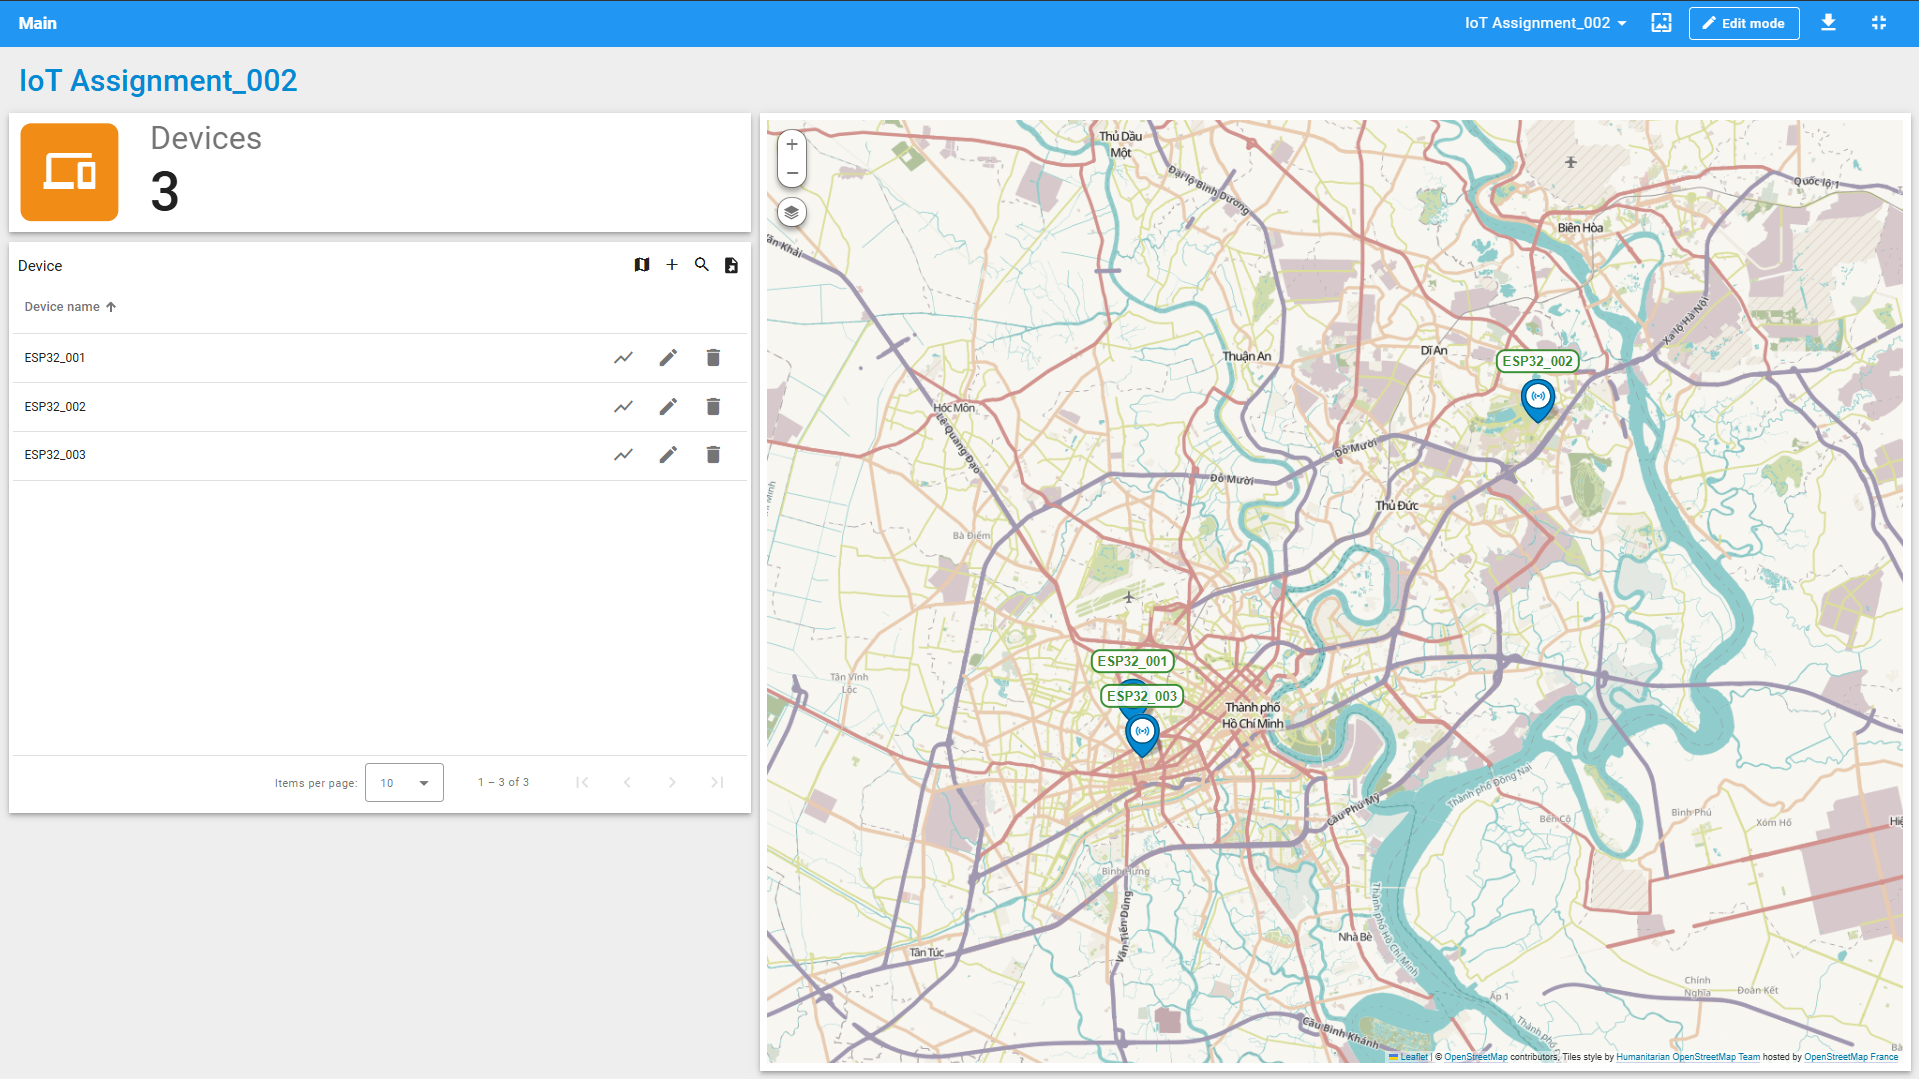
\includegraphics[width=1\textwidth]{pictures/dashboard_001.png}
    \caption{Giao diện mặc định của Dashboard}
\end{figure}


\begin{figure}[H]
    \centering
    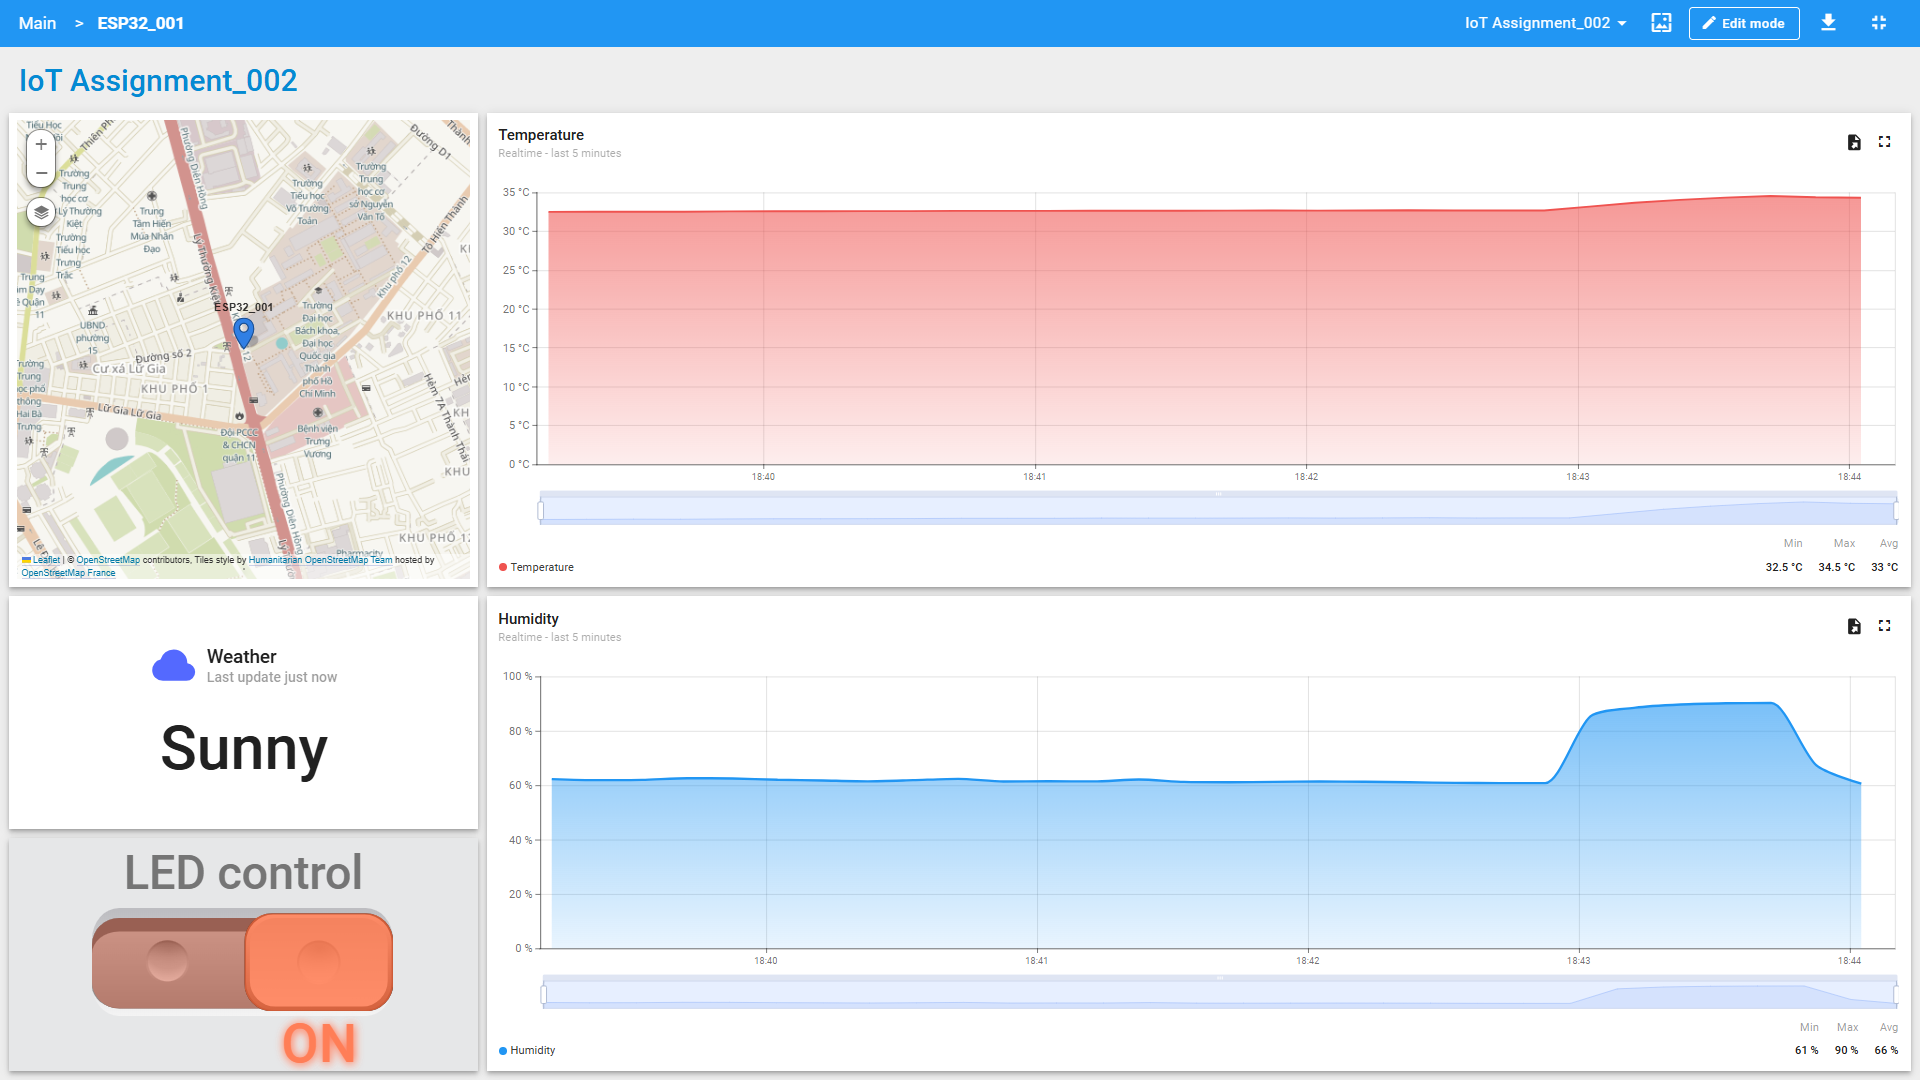
\includegraphics[width=1\textwidth]{pictures/dashboard_002.png}
    \caption{Giao diện Dashboard cho thiết bị ESP32\_001 kết nối với Gateway}
\end{figure}



Dưới đây là các đặc tính kỹ thuật và cấu trúc thành phần của Dashboard "IoT Assignment\_002" với cấu hình chung gồm:

\begin{itemize}
    \item \textit{Giao diện mặc định:} Dashboard được đặt tên là "IoT Assignment\_002" với giao diện mặc định thể hiện các device kết nối với Gateway và vị trí của chúng trên bản đồ, nhằm cho mọi người biết số lượng device cũng như phân bố của chúng.
    \item \textit{Giao diện dữ liệu được gửi từ các device:} Giao diện thứ hai được thể hiện cách thông tin thu thập được từ device như vị trí, nhiệt độ, độ ẩm, kết quả của TinyML. Cùng với đó là sự xuất hiện của một Button gửi tín hiệu RPC về cho ESP32, theo như thiết kế đây là nơi sẽ quyết định LED đơn có bật hay tắt hay không.
\end{itemize}


\subsubsection{Cơ chế gửi email - Rule chain}

Hệ thống điều khiển và giám sát sử dụng công cụ Rule Chain của CoreIOT để thiết lập một quy trình xử lý dữ liệu tự động. Quy trình này không chỉ dừng lại ở việc lưu trữ dữ liệu mà còn thực hiện các phép tính thống kê và gửi báo cáo định kỳ qua Email cho người quản lý. 

\begin{figure}[H]
    \centering
    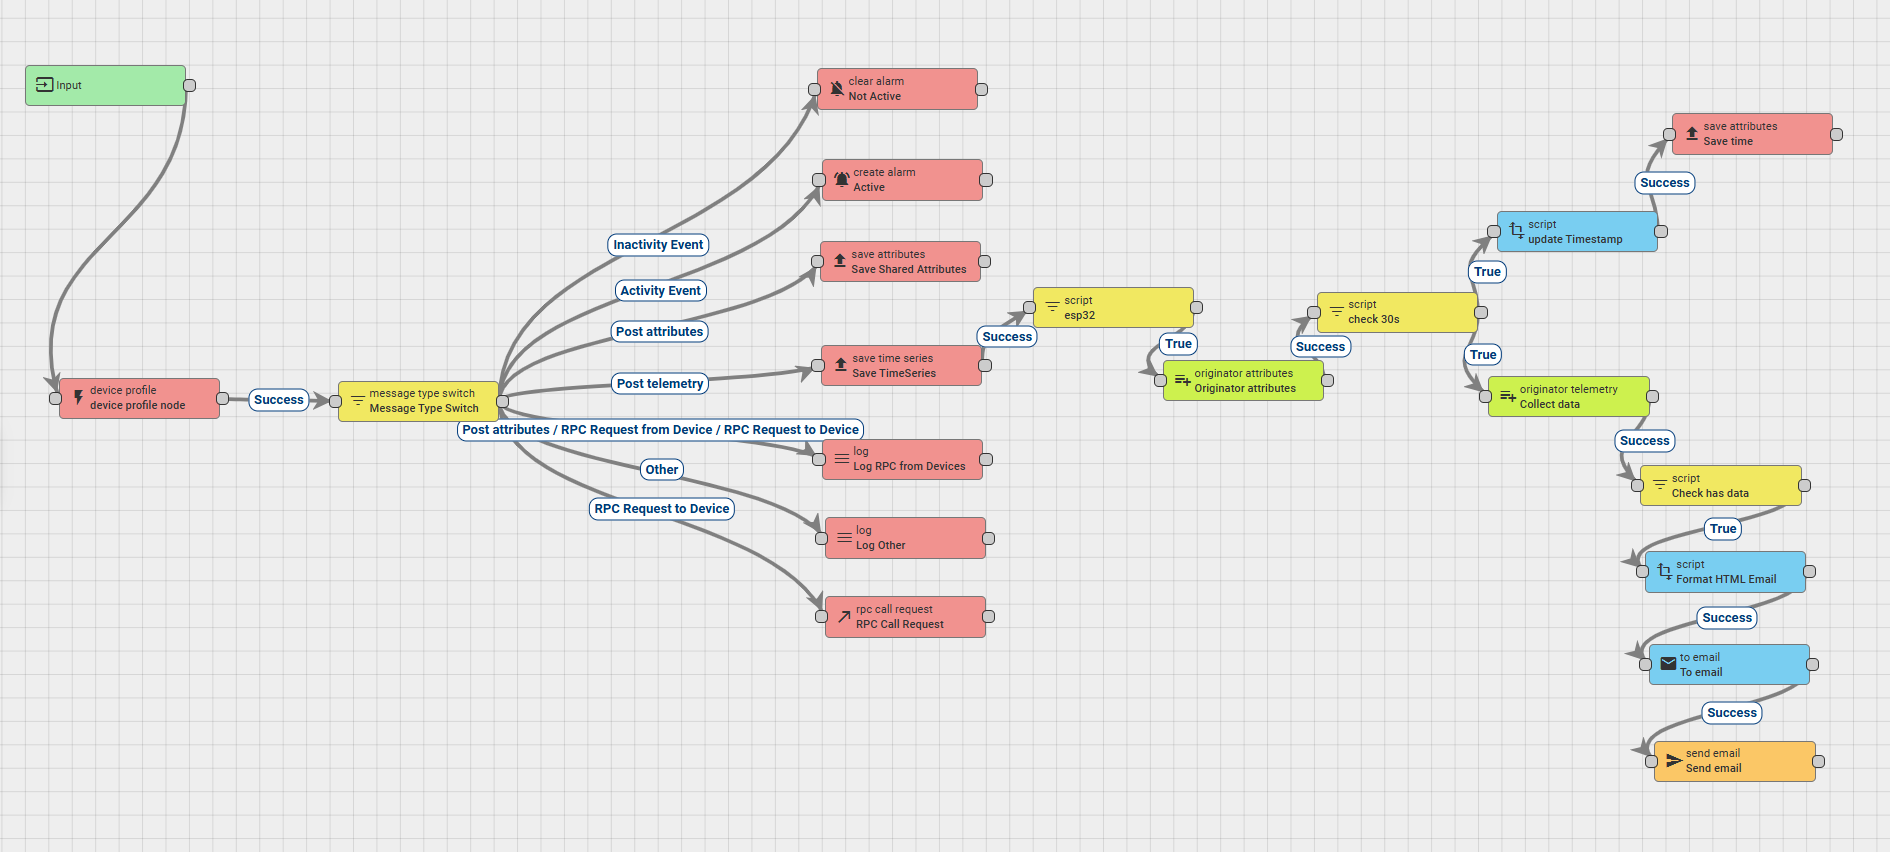
\includegraphics[width=1\textwidth]{pictures/rulechain.png}
    \caption{Rule chain hiện thực cớ chế gửi email}
\end{figure}




Dưới đây là phân tích chi tiết các khối chức năng (Nodes) trong Rule Chain "Gateway":

\begin{itemize}
    \item \textbf{Khối phân loại và lưu trữ cơ sở:}
    \begin{itemize}
        \item \textit{Message Type Switch:} Đây là node điều hướng trung tâm, có nhiệm vụ phân loại các bản tin đến. Các bản tin thuộc loại "Post telemetry" (dữ liệu cảm biến) sẽ được dẫn hướng tới các bước xử lý báo cáo.
        \item \textit{Save TimeSeries:} Thực hiện lưu trữ dữ liệu nhiệt độ, độ ẩm vào cơ sở dữ liệu để hiển thị lên Dashboard. Chỉ khi dữ liệu được lưu thành công, luồng gửi email mới được kích hoạt qua nhánh "Success".
    \end{itemize}

    \item \textbf{Khối lọc thiết bị và kiểm soát tần suất (Rate Limiting):}
    \begin{itemize}
        \item \textit{esp32 (Filter Node):} Sử dụng mã JavaScript để kiểm tra tên thiết bị có phải ESP32 hay không. Điều này đảm bảo hệ thống chỉ xử lý báo cáo cho các node cảm biến ESP32 mà không bị lẫn với các thiết bị khác.
        \item \textit{Originator attributes \& check 30s:} Hai khối này phối hợp để ngăn chặn việc gửi email quá dồn dập. Hệ thống truy xuất thuộc tính \texttt{last\_email\_time} từ server và so sánh với thời gian hiện tại. Theo logic code quy định khoảng cách giữa 2 lần gửi phải $\ge$ 30,000ms.
    \end{itemize}

    \item \textbf{Khối truy vấn và xử lý dữ liệu thống kê:}
    \begin{itemize}
        \item \textit{Collect data:} Khi thỏa mãn điều kiện về thời gian, node này sẽ truy vấn ngược lại cơ sở dữ liệu để lấy toàn bộ các điểm dữ liệu \texttt{temperature} và \texttt{humidity} trong vòng 30 giây gần nhất.
        \item \textit{Check has data:} Kiểm tra mảng dữ liệu trả về. Nếu mảng rỗng (không có dữ liệu trong 30 giây qua), quy trình sẽ dừng lại để tránh gửi email trống.
        \item \textit{Format HTML Email:} Đây là khối xử lý phức tạp nhất bằng JavaScript. Nó thực hiện:
        \begin{itemize}
            \item Chuyển đổi Timestamp sang định dạng giờ Việt Nam (HH:mm:ss).
            \item Tính toán giá trị \textbf{Trung bình (Average)} bằng cách lấy tổng chia cho số lượng mẫu.
            \item Tính toán giá trị \textbf{Trung vị (Median)} bằng cách sắp xếp mảng và lấy giá trị ở giữa.
            \item Xây dựng cấu trúc bảng HTML (\texttt{<table>}) để trình bày dữ liệu chuyên nghiệp.
        \end{itemize}
    \end{itemize}

    \item \textbf{Khối thực thi gửi Email:}
    \begin{itemize}
        \item \textit{To email:} Thiết lập các thông số Header cho email như người gửi, người nhận và tiêu đề thư.
        \item \textit{Send email:} Thực hiện việc gửi thư đi thực tế qua internet.
    \end{itemize}
\end{itemize}

\begin{figure}[H]
    \centering
    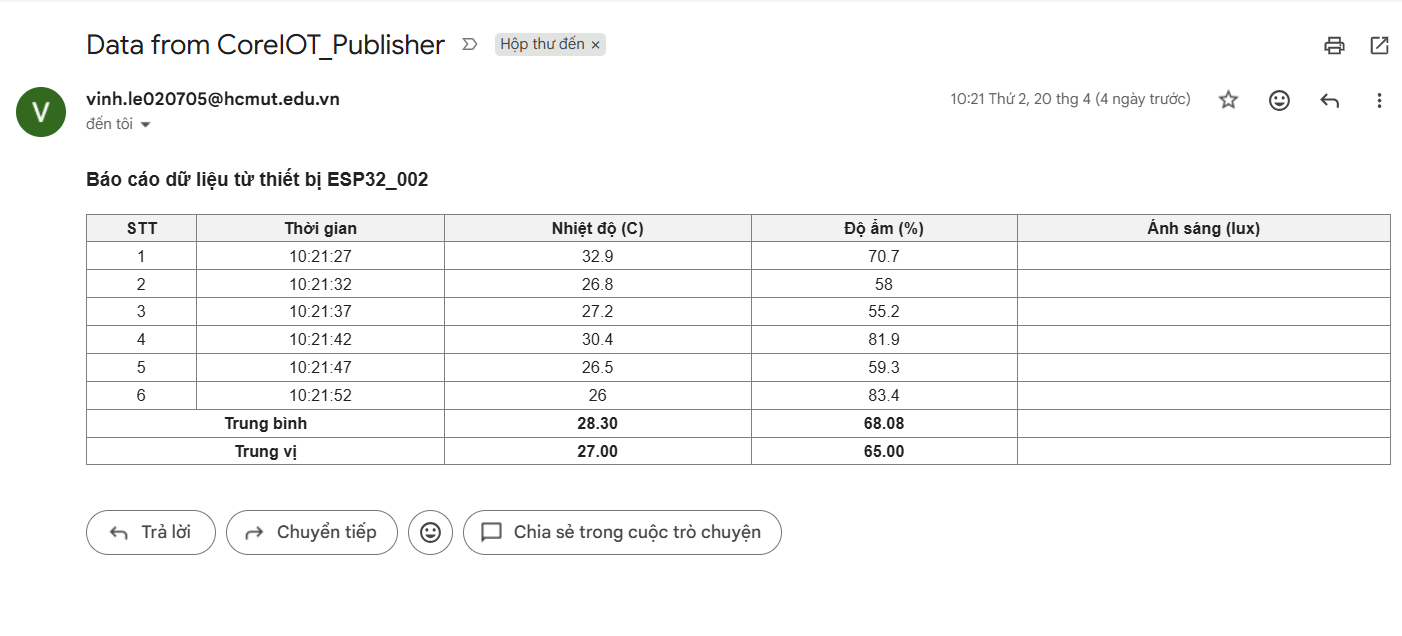
\includegraphics[width=1\textwidth]{pictures/email.png}
    \caption{Email tổng hợp thông tin dữ liệu thu được từ các ESP32}
\end{figure}




\textbf{Đánh giá tổng quan:} Rule Chain này được thiết kế theo mô hình hướng sự kiện (Event-driven). Việc tách biệt luồng cập nhật mốc thời gian và luồng xử lý HTML giúp hệ thống hoạt động ổn định, đảm bảo tính toàn vẹn của dữ liệu báo cáo ngay cả khi lưu lượng dữ liệu từ các node ESP32 gửi về lớn.